\chapter{Architecture}\label{sec:Architecture}
Varroas architecture is organised as a distributed system, whereas there are two main roles in the system: the Agents and the Commander.
The Commander is the central unit that passes work packages of the Scenario to the Agents.
In contrast the Agents process the passed packages and create MQTT clients to execute the testing process.
%The Commander parses the Scenario, splits it into chunks and then distributes it among the agents.

\section{Varroa Distributed System Architecture}
\begin{figure}[h]
	\begin{center}
	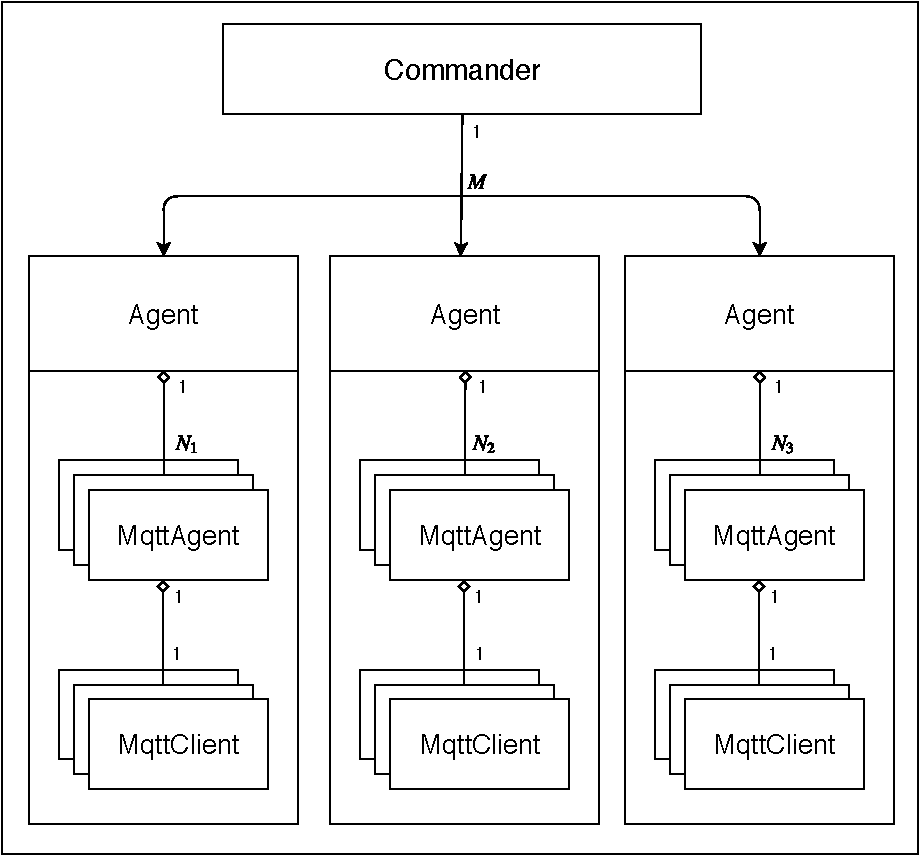
\includegraphics[scale=0.65]{Resources/PDF/Architecture}
	\caption{Varroa Distributed System Architecture}
	\label{pic:Architecture}
	\end{center}
\end{figure}
A Varroa Distributed System is composed of a Commander and multiple Agents.
The Commander and all Agents are executed in separate Varroa Instances.
Every Agent holds a number of MQTT Agents and each MQTT Agent manages one MQTT Client.
\newpage

-\section{Chunk Concept}
A chunk is a work package of the scenario execution designed to be distributed from the Commander to its Agents.
It is then handled by the Agent it is distributed to.
The Agent then creates or uses existing MQTT Agents to execute the Chunk.
It contains:
\begin{itemize}
	\item \textbf{clientCountInChunk}: the amount of clients the chunk represents.
	\item \textbf{clientOffset}: starting index of the clients contained in the chunk.
	\item \textbf{clientGroupId}: identfier for the Client Group contained in the chunk.
	\item \textbf{clientGroupInformation}: contains information concerning the Client Group.
	\item \textbf{commands}: a list of commands that are executed by the clients in the chunk.
\end{itemize}
%\item \textbf{stageDuration}: the duration of the stage this chunk belongs to.
%\item \textbf{lifecycleRate}: the rate at which the contained commands are executed.
%Due to the distributed nature of Varroa it was necessary to be able to spread the information contained in the scenario.
%To secure a deterministic distribution of a scenario's data the chunks had to be evenly spread across the initialized Agents.

\subsection{Chunk Distribution}\label{sec:chunkDistribution}
\begin{figure}[h]
	\begin{center}
	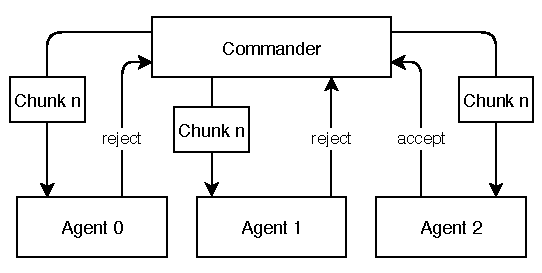
\includegraphics[scale=1.2]{Resources/PDF/ChunkDistribution}
	\caption{Distribution of a Chunk}
	\label{pic:ChunkDistribution}
	\end{center}
\end{figure}
A Chunk is deterministically assigned to an Agent to ensure that it gets executed by the same Agent even on multiple runs of the scenario. This determinism is needed to avoid fluctuation of reporting results that would be caused by Varroa and not the MQTT system under test.
%To secure a deterministic execution of a scenario the every chunk needs to be distributed to the same Agent in every execution of the scenario.
To ensure this determinism a round-robin distribution of the scenario's Chunks combined with a handshake mechanism is used:
In accordance to figure \ref{pic:ChunkDistribution} the Commander tries to distribute a Chunk to an Agent who then answers with an accept or reject.
If the Agent rejects the Chunk (see figure \ref{pic:RejectHandshake}) the Commander then tries to distribute the Chunk to the next Agent in the same manner until one Agent accepts.
When accepting the Chunk the Agent waits for a Start Message from the Commander and upon receiving it the Agent starts executing the Chunk.
After a successful execution of the Chunk the Agents sends a Finished Message to the Commander (see figure \ref{pic:AcceptHandshake}).


\begin{minipage}[ht]{0.48\textwidth}
	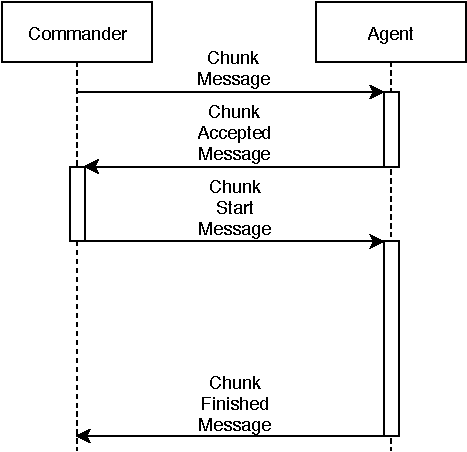
\includegraphics[width=\textwidth]{Resources/PDF/ChunkAcceptedHandshake}
\end{minipage}
\hfill
\begin{minipage}[ht]{0.48\textwidth}
	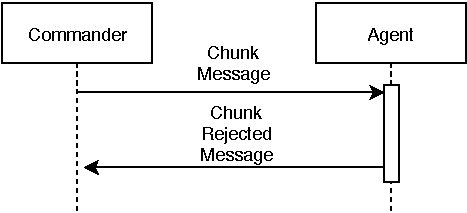
\includegraphics[width=\textwidth]{Resources/PDF/ChunkRejectHandshake}
\end{minipage}

\begin{minipage}[ht]{0.48\textwidth}
	\captionof{figure}{Chunk Handshake with Accept}
	\label{pic:AcceptHandshake}
\end{minipage}
\hfill
\begin{minipage}[ht]{0.48\textwidth}
	\captionof{figure}{Chunk Handshake with Reject}
	\label{pic:RejectHandshake}
\end{minipage}
